\documentclass[a4paper,10pt]{article}
\usepackage[french]{babel} 
\usepackage[utf8]{inputenc}
\usepackage{graphicx}

\newcommand{\rubic}{Rubik's Cube}
\newcommand{\asi}{Architecture des Systèmes d'Information}

\title{ECAO : Reconnaissance d'images appliqué au \rubic}
\author{Delphine SOULA \& Gabriel WIART}

\begin{document}

 \maketitle
%%%%%%%%%%%%%%%%%%%%%%%%%%%%%%%%%%%%%%%%%%%%%%%%%%%%%%%%%%%%%%%%%%%%%%%%%%%%%%%%%
\section{Introduction} % P0
  Le but de cette UV est de compléter le travail de résolution du \rubic{} effectué par nos camarades au cours des semestres précédents en 
y ajoutant un module de reconnaissance de formes. 
  Ce module aura pour but de reconnaître la configuration de départ du \rubic{} afin de rendre totalement automatisée la chaîne d'acquisition. 

  Nous allons diviser cette tache en trois tâches successives : 
\begin{enumerate}
  \item Recalage permettant de trouver les carrés de la face considérée,  
  \item Détection des couleurs à partir des images de la webcam couleur, 
  \item Interfaçage avec le système de résolution déjà existant en Java. 
\end{enumerate}

  Nous avons choisi de traiter ce sujet car nous voulions approfondir et mettre en application les notions de traitement d'images 
et reconnaissance de forme. 
  De plus, l'automatisation du robot permettrait de mettre en valeur le travail des élèves du département 
\asi{} par la finition de la chaîne de traitement des données aboutissant à la résolution du \rubic{}. 

  Nous avons travaillé sur des images prises grâce à une webcam fixée sur le robot. 
Nous avons ainsi récupéré les différentes face du \rubic{} avec des conditions environnementales notamment d'éclairage différentes. 

  Nous avons choisi de travailler sur ces images sous Octave. 
En effet, l'outil Octave est étudié pour optimiser la manipulation des matrices et est libre, 
c'est pour cela que nous avons choisi cet outil de développement. 

  Nous allons dans la suite de ce rapport vous décrire notre démarche et justifier nos choix pour chacune des trois tâches 
décrites ci-dessus. 


%%%%%%%%%%%%%%%%%%%%%%%%%%%%%%%%%%%%%%%%%%%%%%%%%%%%%%%%%%%%%%%%%%%%%%%%%%%%%%%%%
\section{Détection des contours} % P1
  La première étape est le recalage de l'image permettant de trouver les carrés de la face considérée. 

  Pour cela, nous avons étudié et comparé différentes façons de trouver les contours du \rubic{} : 
\begin{itemize}
  \item Faire une rotation de l'image pour recadrer l'image, 
  \item Étudier les projetés en X et Y des couleurs des points de l'image pour trouver les lignes de points 'noirs' caractéristiques des 
contours : 
    \begin{itemize}
      \item Par l'étude de la dérivée, 
      \item Par la recherche par seuil, 
      \item Par l'étude de la variance des N points successifs. 
    \end{itemize}
  \item Étudier la variation sur une fenêtre de points de l'image. 
\end{itemize}

  Nous avons travaillé sur une image en niveaux de gris car l'information sur les couleurs n'était pas intéressante pour cette étude. 
Nous avons obtenu l'image en niveaux de gris grâce aux fonctions \textbf{imread} et \textbf{rgb2gray} disponible sous octave. 


\subsection{Recherche de la meilleure rotation}
Avant de pratiquer une détection des faces du cube, nous recherchons l'orientation idéale pour permettre la récupération d'informations via des projections de l'image en abscisses et ordonnées. Pour cela, les arêtes du cube doivent être parallèles aux arêtes de l'image.

La projection de l'image en ordonnées est un vecteur contenant les moyennes pondérées des pixels de chacune des lignes, et la projection en abscisses correspont à la moyenne pour chacune des colonnes.

Afin d'effectuer la transformation, nous utilisons la méthode suivante :
L'orientation idéale du cube se caractérise, sur les projections de l'image en abscisses et ordonnées, par la maximisation des pics correspondant aux arêtes sombres du cube.

La méthode est la suivante : nous effectuons plusieurs rotations matricielles sur l'image d'origine. Nous effectuons ensuite les projections en abscisses et en ordonnées pour chaque rotation et nous retenons la rotation dont les pics sont maximaux.



\subsection{Utilisation de la dérivée}
% Delphine 

  Nous avons pensé à étudier les contours grâce aux projections en X et en Y de l'image. 
L'idée est de faire apparaître les pics de pixel noir au niveau des contours. 

  Afin de retrouver algorithmiquement les positions des lignes verticales et horizontales qui définissent les carrés du \rubic{}, 
nous avons décidé de dériver les projections afin de déduire les positions en X et en Y de ces lignes. 

\subsubsection*{Principe de la méthode} 

  Cette méthode est basée sur l'étude de la dérivée. 
Elle suit les étapes suivantes : 
\begin{enumerate}
  \item Trouver les extremums. 

  L'étude du signe de la dérivée nous permet de localiser les extremums. 
En effet, leurs positions correspondent aux endroits où la dérivée change de signe, c'est à dire passe par zéro. 
Comme la dérivée a très peu de chance de valoir zéro, nous avons étudié le changement de signe de celle-ci. 

  Nous obtenons les positions de tous les extremums. 

  \item Trouver les minimums. 

  Les changements de signe dans le cas de minimum vont passer d'un signe positif à un négatif de la dérivée. 
Ainsi, nous avons récupéré sur l'ensemble des positions des extremums précédemment identifiés uniquement celles qui 
correspondent à la valeur 1 sur le vecteur caractéristique du signe de la dérivée. 

  Nous obtenons les positions de tous les minimums locaux. 

  \item Trouver le bon nombre de minimum en respectant une distance définie entre chacun de ces minimums. 
 
La méthode consiste à remplir une liste d'indices initialement vide avec les positions de minimum intelligemment choisies : 
  \begin{itemize}
    \item On récupère le minimum du vecteur en entrée dont l'indice correspond aux positions possibles, 
    \item Si la liste d'indices est vide, on l'ajoute; 
Sinon on calcule la distance minimale entre lui et les positions déjà contenues dans la liste d'indices 
et on la compare à celle qui définie la condition de distance voulue entre les minimums : 

  Si le distance calculée est supérieure, la position est ajoutée à la liste d'indices ; Sinon, non. 
    \item Afin que ce minimum ne soit plus considéré au cours des futures itérations, 
on modifie la valeur du vecteur à cette position tel qu'il prennent la valeur maximale de ce vecteur. 
  \end{itemize}
\end{enumerate}

  La signature de la fonction créée est la suivante : \\
\textit{function [indicePicMin]=detectionPicDerivee(VecteurEtudie, nbPic, largeurPic)}

\subsubsection*{Résultats obtenus par cette méthode}

     La figure~\ref{derivee_resultat_1} présente le résultat obtenu sur une image orientée et ayant subit un filtrage avec la méthode de la dérivée : 
 
 \begin{figure}[!h]
 \centering
 %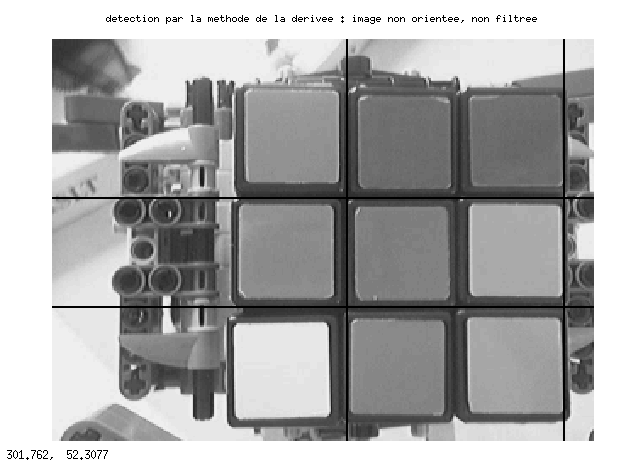
\includegraphics[width=0.45\linewidth]{Images/Derivee_img_traitement_1.png} 
 %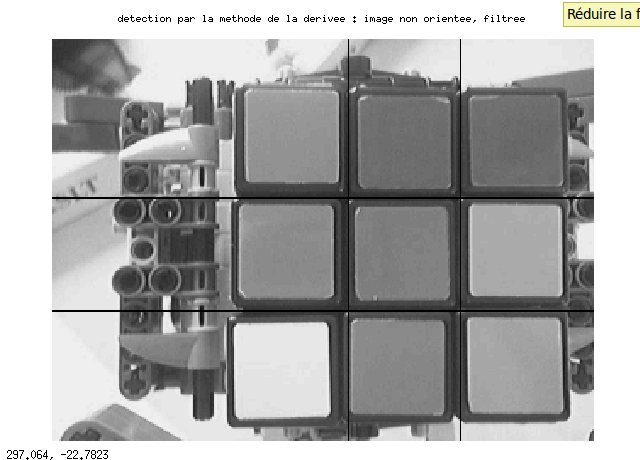
\includegraphics[width=0.45\linewidth]{Images/Derivee_img_traitement_2.png} \\
 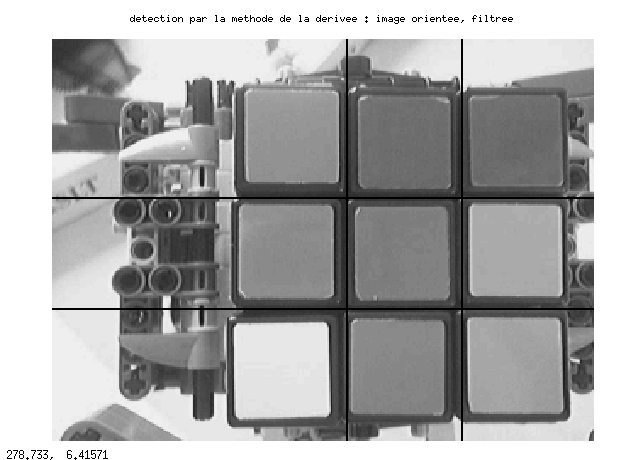
\includegraphics[width=0.9\linewidth]{Images/Derivee_img_traitement_3.png} 
 %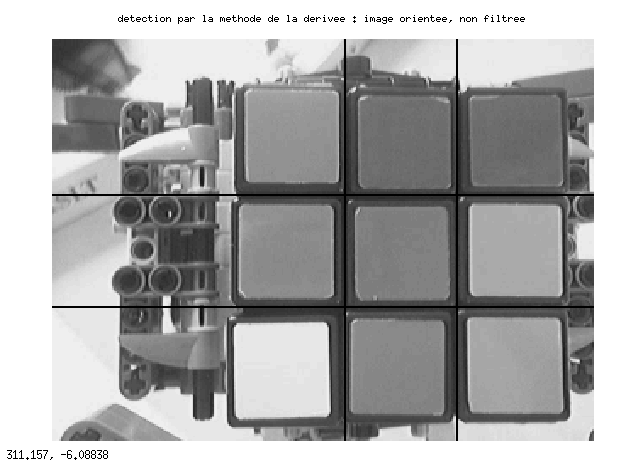
\includegraphics[width=0.45\linewidth]{Images/Derivee_img_traitement_4.png} 
 \caption{Résultat de la méthode dérivée} 
 \label{derivee_resultat_1}
 \end{figure}


\subsection{Utilisation de la barre de seuillage}
% Gabriel

\subsubsection*{Principe de la méthode} 

Cette méthode part du constat suivant : les facettes colorées du cube sont séparées par une zone nettement plus sombre. Cette zone se caractérise par l'apparition de pics sur les projections en abscisses et ordonnées. 

Dans un premiers temps nous avons fixé manuellement un seuil pour délimiter les facettes colorées. Nous nous sommes rapidement rendus comte que le seuil fixe ne pouvait convenir à des images dont les conditions d'éclairage varient. 

Nous avons donc réalisé un algorithme de détection de seuil dont le principe est le suivant : Nous commençons par fixer un seuil à la valeur la plus sombre de la projection.

Ensuite nous éclairsissons la valeur de ce seuil jusqu'à croiser un minimum de deux pics distincts.

\subsubsection*{Résultats obtenus par cette méthode}
 
 Nous réalisons par exemple un seuillage sur la courbe suivante (figure \ref{projX}):
 \begin{figure}[!h]
 \centering
 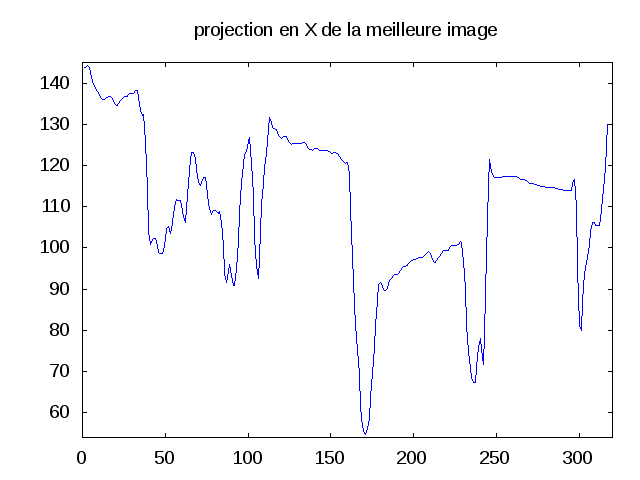
\includegraphics[width=0.60\linewidth]{Images/projX.png}
 \caption{projetée en abscisses} 
 \label{projX}
 \end{figure}
 
 Nous pouvons notament obtenir le résultat suivant (figure \ref{barreGlissante}):
\begin{figure}[!h]
 \centering
 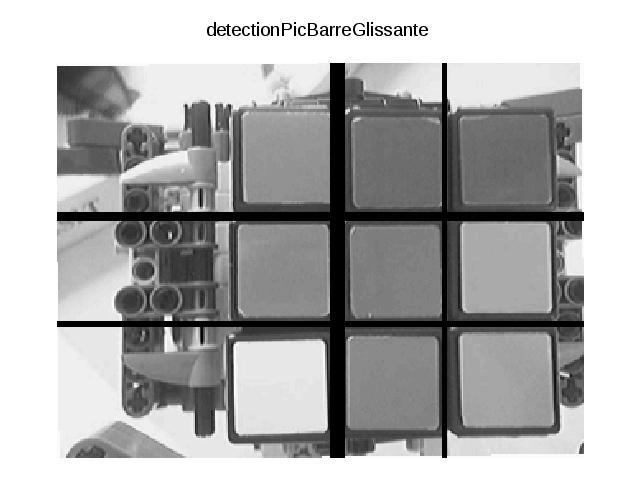
\includegraphics[width=0.60\linewidth]{Images/detectionBarreGlissante.png}
 \caption{détéction par la méthode de la barre de seuillage} 
 \label{barreGlissante}
 \end{figure}


\subsection{Utilisation de la variance des projectetés en X et Y} 
  On remarque que sur les courbes des projections de l'image en X et en Y, la courbe marque des paliers au 
niveau des carrés du \rubic{}. 

  Étant donné que la couleur est fortement corrélée sur ces paliers, nous avons décidé d'étudier la variance sur 
un nombre défini de points successifs de ces courbes et d'en extraire des plats caractéristiques de ces paliers. 

\subsubsection*{Principe de la méthode} 

  Cette méthode étudie la variance des vecteurs de projection en X et Y de l'image. 

Afin de la mettre en place, nous avons créé une méthode intermédiaire qui permet de calculer un vecteur contenant les valeurs de la variance 
du vecteur en entrée sur un nombre de points successifs défini. 

La méthode générale suit les étapes suivantes : 
\begin{enumerate}
  \item Calcule de la variance du vecteur de projection en entrée grâce à la fonction décrite précédement. 
  \item Recherche du seuil tel que l'on ait un nombre de plat calculé inférieur ou égal à un nombre voulu. 

Nous faisons le choix d'initialiser un seuil à $\frac{1}{4}$ de la valeur maximale du vecteur en entrée 
et de fixer le pas de modification de ce seuil à $-\frac{1}{10}$ de cette valeur. 
%On initialise la valeur de retour de façon a ce qu'elle vérifie la condition d'entrée dans l'itération suivante : 
\begin{itemize}
  \item On note X la largeur maximale d'un plat. 
Afin d'optimiser l'algorithme et pour garantir une distance minimum entre les plats recherchés, nous avons 
établi que l'indice de parcours de la variance étudiée commence à X et avance par pas de $\frac{X}{2}$ jusqu'à la fin du vecteur 
variance moins la valeur $\frac{X}{2}$. 
  \item On considère qu'un plat existe quand la moyenne de X valeurs successives du vecteur de variance est inférieure au seuil. 
Nous concervons dans un vecteur les indices vérifiant cette condition.
La taille de ce vecteur est la condition de sortie de l'itération.  
  \item Le seuil est diminué de la valeur d'un pas de seuil à chaque itération. 
\end{itemize}

  \item Si le nombre de plat contenus dans le vecteur est égal au nombre voulu, on a le résultat ; 
Sinon, nous récupérons la valeur du vecteur contenant les indices des plats à l'itération précédente et 
nous y supprimons successivement les valeurs les plus semblables aux autres afin d'avoir le nombre de plats souhaité. 

  La distance que nous avons choisi pour calculer la matrice de distance entre ces valeurs et déterminer leur pertinence,
est la distance euclidienne. 
\end{enumerate}

  Les signatures des fonctions créées sont les suivantes : 
\begin{itemize}
  \item \textit{function [variancefinale] = varianceCoordonnee(vecteur, longueurVariance)}
  \item \textit{function [plat] = detectionPlatVariance1D(vecteur, longueurVariance, nombreDePlat, largeurPlat)}
\end{itemize}

\subsubsection*{Résultats obtenus par cette méthode}

     La figure~\ref{variance_resultat_1} présente le résultat obtenu sur une image orientée et ayant subit un filtrage avec la méthode de la variance 1D : 
 
 \begin{figure}[!h]
 \centering
 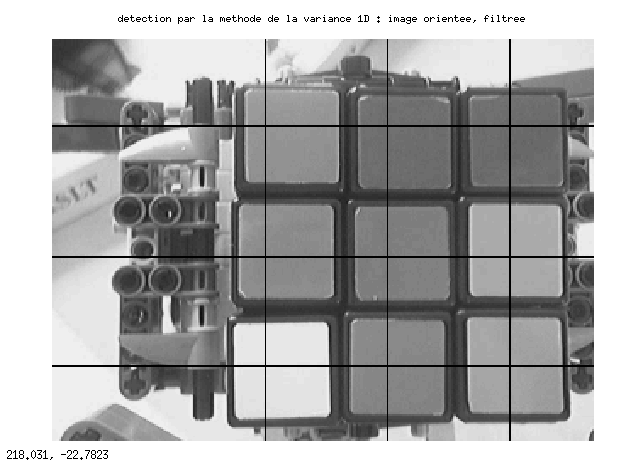
\includegraphics[width=0.9\linewidth]{Images/Variance1D_img_traitement.png} 
 \caption{Résultat de la méthode variance 1D} 
 \label{variance_resultat_1}
 \end{figure}


\subsection{Utilisation de la variance sur la matrice de l'image} 
  Afin de détecter les carrés du \rubic{}, nous avons étudié la variance entre les points voisins de l'image. 
En faisant l'hypothèse que les carrés du cube sont là où la variance varie le moins dans l'image. 

\subsubsection*{Principe de la méthode} 

  Contrairement aux images précédentes, nous travaillons directement avec l'image sans utiliser les projections en X et en Y. 

Cette méthode peut se décomposer en plusieurs étapes : 
\begin{enumerate}
  \item Calcul de la variance de l'image : \\
  Nous déterminons un entier qui correpond à la taille (hauteur et largeur) de la fenêtre qui va parcourir l'image. 
La variance est calculée sur chacune de ces fenêtres pour obtenir une matrice contenant les variances sur toutes ces fenêtres. 

On obtient une matrice qui est représentée comme dans la figure~\ref{variance2D_VARavant}. 

\begin{figure}[!ht]
\centering
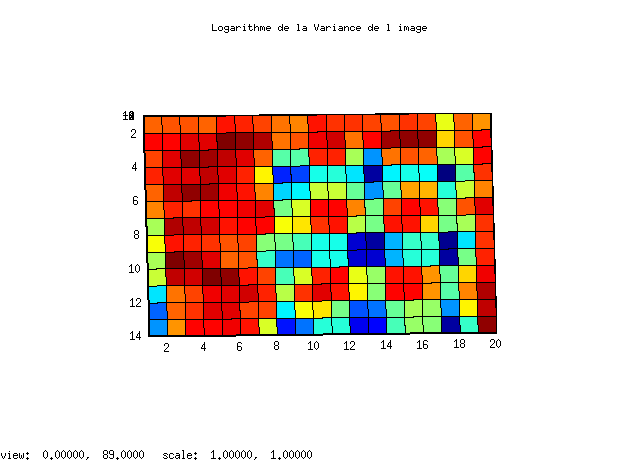
\includegraphics[width=\linewidth]{Images/Variance2D_variance_avan_2.png}
\caption{Variance obtenue pour l'image conf4/face4}
\label{variance2D_VARavant}
\end{figure}

  Pour rappel, le bleu correspond aux valeurs de variance les plus faibles alors que le rouge correspond aux valeurs élevées.
On voit apparaître les faces du \rubic{}. 

  On remarque cependant qu'il y a en bas à gauche, un zone bleue qui peut poser problème lors de la détection des plats. 

  \item Recherche des plats : \\
 
  Pour rechercher les plats, on a pris les minimums de variance successifs de la matrice de Variance sachant que pour chaque minimum détécté, nous avons changé sa valeur et celle de ces voisins afin que ce plat ne soit pas détécté à l'itération suivante. 

  Un plat est donc représenté par un point ayant des coordonnées X et Y et qui correspond à l'estimation du centre du carré du \rubic.

 La matrice modifiée devient la figure~\ref{variance2D_VARapres}. 

\begin{figure}[!ht]
\centering
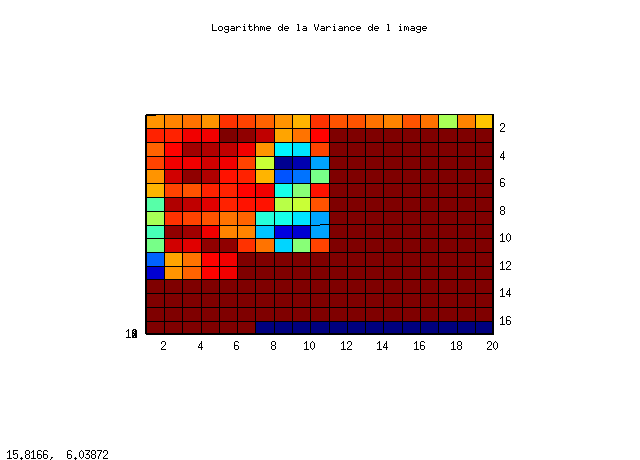
\includegraphics[width=\linewidth]{Images/Variance2D_variance_apres_2.png}
\caption{Variance obtenue pour l'image conf4/face4}
\label{variance2D_VARapres}
\end{figure}

  Nous pouvons constater que la zone qui posait problème précédemment a bien été séléctionnée comme un plat. 
Il faut donc faire un tri qui permettrait de détecter ce genre d'erreur. 

  \item Tri des plats : \\ 

  Pour trier les plats, nous avons utilisé la matrice de distance entre les plats. 
Nous avons fait notre choix de garder ou supprimer un plat en fonction de sa distance mimimale avec les autres plats. 
Ainsi tous les plats dont cette distance est inférieure à un seuil sont supprimés. 
Plus ce seuil est faible, plus il nous réduit le critère d'alignement des points. 

  Ce critère est appliqué pour chaque plat sur leurs absisses et leurs ordonnées. 

  \item Interpolation des plats manquants : \\

  Nous avons maintenant un nombre de plat inférieur à celui dont nous avons besoin pour retrouver les 9 carrés du \rubic{}. 

  Nous avons pour résoudre ce problème diviser l'image du cube en plusieurs zones qui correspondent aux emplacements les plus succeptibles de contenir une face. 
  Ce découpage en zone est défini comme présenté dans la figure ~\ref{variance2D_zone}. 

\begin{figure}[!ht]
\centering
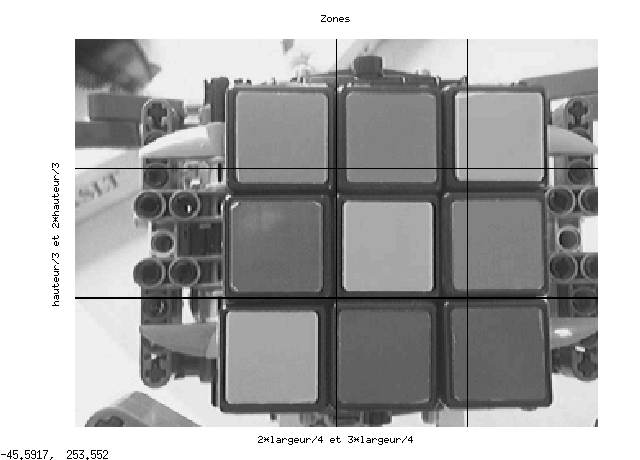
\includegraphics[width=\linewidth]{Images/Variance2D_zone.png} 
\caption{Zone de probabilité d'apparition d'une face} 
\label{variance2D_zone}
\end{figure}

  Pour ajouter des points nous avons récupérer grâce à la fonction \textit{unique} les coordonnées X et Y des plats validés. 
Nous avons noté lX et lY le nombre d'absisse et le nombre d'ordonnée appartenant à des plats validés et nous avons traité les cas suivants : lX égale 1, 2, 3 ou 4 et lY égale 1, 2, 3 ou 4. 
De plus, on note dX et dY la distance minimale entre les plats restants qui est l'approximation de la distance entre deux plats voisins. 

Les cas pour lX ont été traités de la façon suivante : 
  \begin{itemize}
    \item $lX=1$ : En fonction de la zone où est le plat valide, on ajoute deux plats de même absisse dans les zones libres tel qu'il y ait une distance dY entre ces points . 
    \item $lX=2$ : En fonction de la zone où sont les plats valides, on ajoute un dernier plat de même absisse dans la zone libre tel qu'il y ait une distance dX entre ces points . 
    \item $lX=3$ : On garde ces trois plats valides. 
    \item $lX=4$ : On a décidé de supprimer un plat dont la distance minimale avec les autres plats est la plus grande. 
  \end{itemize}

  Cependant si lX et lY valent 1 ou si une de ces deux variables est suppérieure à 4, la fonction renvoie une erreur. 
De même, si un plat est ajouté alors que ces coordonnées approximés sortent de l'image, une erreur est retournée. 
\end{enumerate}

  La signature de la fonctions créée est la suivantes : \\
\textit{function [plat, erreur] = detectionPlatVariance2D\_coord(image, largeurFenetre)}


\subsubsection*{Résultats obtenus par cette méthode}

  Les figures~\ref{variance2D_resultat_1} et ~\ref{variance2D_resultat_2} présentent les résultats obtenus pour deux images avec la méthode de la variance 2D : 

\begin{figure}[!ht]
\centering
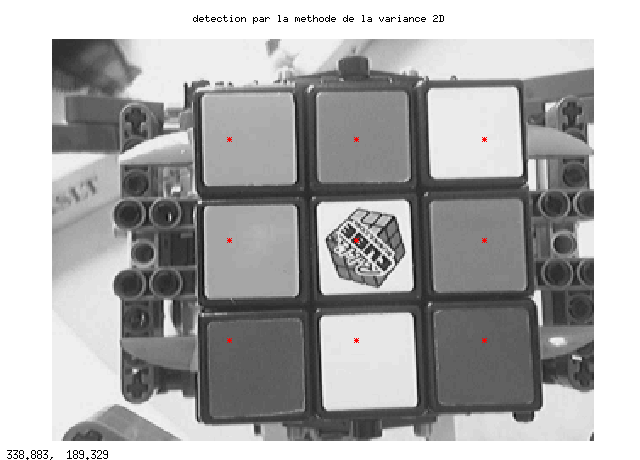
\includegraphics[width=0.6\linewidth]{Images/Variance2D_img_apres_1.png} 
\caption{Résultat de la méthode variance 2D} 
\label{variance2D_resultat_1}
\end{figure}

\begin{figure}[!ht]
\centering
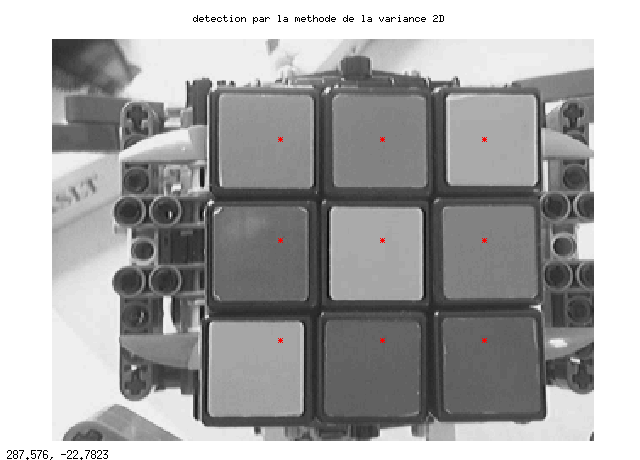
\includegraphics[width=0.6\linewidth]{Images/Variance2D_img_apres_2.png}
\caption{Résultat de la méthode variance 2D} 
\label{variance2D_resultat_2}
\end{figure}

  On remarque que les résultats sont exacts lorsque l'on est dans le cas de la face blanche ``spéciale'',de la face orientée et de celle non-orientée. 
  Cependant la face ayant des reflets obtient de mauvais résultats. 


\subsection{Comparaison des différentes méthodes}
  Nous avons comparé ces différentes méthodes afin de choisir la plus appropriée à nos besoins. 

  Afin de tester la performance de chacune de ces méthodes, nous avons testé chacune d'elle sur un échantillon de photo de 5 lots de 6 faces avec des prétraitements différents.

\subsection*{Etude des pré-traitements adaptés pour chaque méthode}

  Dans ce paragraphe, nous allons présenté les choix des pré-traitements le mieux adaptés à chacune des méthode précédemment étudiées. 

%%%%%%%%%%%%%%%%%%%%%%%%%%%%%%%%%%%%%%%%%%%%%%%%%%%%%%%%%%%%%%%%%%%%%%%%%%%%%%%%%%%%%%%%%%%%%%%%%%%%%%%%%%%%%%%%%%%%%%%%%%%%%%%%%%%%%%%%%%%%%%%%%%%%%%%%%%%%%%%% DERIVEE
  Voilà les résultats obtenus pour cet échantillon par la méthode de la dérivée : \\
\begin{tabular}{|c|c|c|c|c|}
  \hline
 \textbf{Prétraitement} & NF + NO & F + NO & NF + O & F + O  \\
  \hline
  OK & 89\% & 94\% & 83\% & 94\% \\ % conf 4 5 6 
  OKR & 45\% & 55\% & 25\% & 25\% \\  % conf 7 8
  \hline 
\end{tabular}

F = utilisation d'un filtre, NF = pas d'utilisation d'un filtre, O = image orientée, NO = image non orienté \\
OK = nombre d'image où la détection des contours est un succés, OKR = nombre d'image ayant des reflets où la détection des contours est un succés\\

Nous comptons comme succes le fait de trouver les deux séparations centrale entre les facettes
  
  Nous constatons que cette méthode donne généralement de bon résultats. En effet la majore partie des échecs sont du à la détection d'une arrète du cube au lieux d'une séparation.  % A remplir 


%%%%%%%%%%%%%%%%%%%%%%%%%%%%%%%%%%%%%%%%%%%%%%%%%%%%%%%%%%%%%%%%%%%%%%%%%%%%%%%%%%%%%%%%%%%%%%%%%%%%%%%%%%%%%%%%%%%%%%%%%%%%%%%%%%%%%%%%%%%%%%%%%%%%%%%%%%%%%%%% SEUILLAGE
  Voilà les résultats obtenus pour cet échantillon par la méthode du seuillage : \\
\begin{tabular}{|c|c|c|c|c|}
  \hline
 \textbf{Prétraitement} & NF + NO & F + N0 & NF + 0 & F + 0  \\
  \hline
  OK & 100\% & 94\% & 89\% & 100\% \\ % conf 4 5 6 
  OKR & 83\% & 83\% & 83\% & 75\% \\ % conf 7 8
  \hline 
\end{tabular}

F = utilisation d'un filtre, NF = pas d'utilisation d'un filtre, O = image orientée, NO = image non orienté \\
OK = nombre d'image où la détection des contours est un succés, OKR = nombre d'image ayant des reflets où la détection des contours est un succés\\

Nous comptons comme succes le fait de trouver au moins les deux séparations centrales des facettes.

 Nous constatons que les résultats sont glogalement bon. Cependant il apparait un bruit sous la forme d'une zone sombre parazite qui peut être très genant pour la suite tu travail.


%%%%%%%%%%%%%%%%%%%%%%%%%%%%%%%%%%%%%%%%%%%%%%%%%%%%%%%%%%%%%%%%%%%%%%%%%%%%%%%%%%%%%%%%%%%%%%%%%%%%%%%%%%%%%%%%%%%%%%%%%%%%%%%%%%%%%%%%%%%%%%%%%%%%%%%%%%%%%%%% VARIANCE 1D 
  Voilà les résultats obtenus pour cet échantillon par la méthode de la variance sur les projections en X et Y : \\
\begin{tabular}{|c|c|c|c|c|}
  \hline
 \textbf{Prétraitement} & NF + NO & F + N0 & NF + 0 & F + 0  \\
  \hline
  OK & 0\% & 0\% & 0\% & 0\% \\ % conf 4 5 6 
  OKR & 0\% & 0\% &  0\% & 0\% \\ % conf 7 8
  \hline 
\end{tabular}

F = utilisation d'un filtre, NF = pas d'utilisation d'un filtre, O = image orientée, NO = image non orienté \\
OK = nombre d'image où la détection des contours est un succés, OKR = nombre d'image ayant des reflets où la détection des contours est un succés\\

Nous comptons comme succes le fait que chaques intersection tombe sur une facette colorée.

  En vue des résultats obtenus, nous pouvons clairement dire que cette méthode ne se suffit pas à elle même. Cependant, il est possible de combiner cette approche avec la méthode de la dérivé en vu d'amméliorer ces résultats.

%%%%%%%%%%%%%%%%%%%%%%%%%%%%%%%%%%%%%%%%%%%%%%%%%%%%%%%%%%%%%%%%%%%%%%%%%%%%%%%%%%%%%%%%%%%%%%%%%%%%%%%%%%%%%%%%%%%%%%%%%%%%%%%%%%%%%%%%%%%%%%%%%%%%%%%%%%%%%%%% VARIANCE 2D 
  Voilà les résultats obtenus pour cet échantillon par la méthode de la variance sur l'image : \\
\begin{tabular}{|c|c|c|}
  \hline
 \textbf{Prétraitement} & NO & 0  \\
  \hline
  OK & 55\% & 55\%  \\ % conf 4 5 6 
  OKR & 0\% & 0 \% \\ % conf 7 8
  \hline 
\end{tabular}

O = image orientée, NO = image non orienté \\
OK = nombre d'image où la détection des contours est un succés, OKR = nombre d'image ayant des reflets où la détection des contours est un succés\\

  Ces résultat montrent que cette méthode implémenté seule ne permet pas une detection correcte des facettes du cube.

  


%%%%%%%%%%%%%%%%%%%%%%%%%%%%%%%%%%%%%%%%%%%%%%%%%%%%%%%%%%%%%%%%%%%%%%%%%%%%%%%%%
\section{Recherche des couleurs} % P2
  La seconde partie de notre projet à consisté à initialiser les couleurs sur les cases précédement détéctées du cube. 

  Pour cela, nous avons créé sous matlab la structure suivante : 
\begin{itemize}
  \item Cube = 6 Face ; 
  \item Face = 2 Images orientées du cube l'une colorée l'autre en niveau de gris, 1 vecteur de projection en X et 1 en Y, 9 Carre, 1 Centre, 1 Variation centre ; 
  \item Carre = 4 Points définissant une zone de calcul, 1 Centre, 1 vecteur RGB contenant la couleur moyenne calculée sur la zone caractéristique du carré ; 
  \item Centre = 1 Point ; 
  \item Point = Coordonnées (X,Y). 
\end{itemize}

  Pour initialiser nos algorithmes de reconnaissance de couleur, nous nous sommes servi des informations extraites de chacun des 6 centres des faces du cube. 
  En effet, nous savons que chaque centre est caractéristique d'un ensemble de 9 carrés d'une même couleur. 

  Nous allons donc faire de la classification pour mettre en valeur 6 groupes de 9 carrés en utilisant les valeurs RGB comme caractéristiques. 
  Nous utilisons la valeur moyenne des valeurs RGB sur une zone représentative du carré dont le centre est trouvé grâce à la méthode de la détection de contour. 

  La figure~\ref{fig:RGB_init} est celle des valeurs RGB des différents carrés, centres inclus. 
  \begin{figure}[!ht]
    \centering
    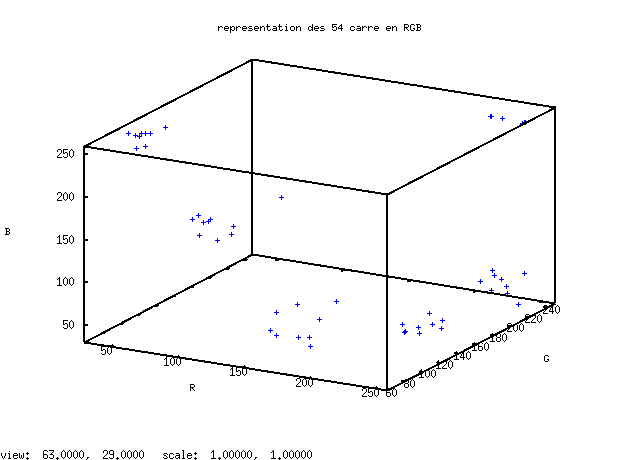
\includegraphics[width=0.5\linewidth]{./Images/RGB_init.png}
    \caption{Représentation des données RGB des différents carrés}
    \label{fig:RGB_init}
  \end{figure}

  \subsection*{Détection du centre blanc}

  Le \rubic{} que nous utilisons pour la reconnaissance a un dessin sur la face blanche, ainsi nous ne pouvons pas l'utiliser les informations de ce centre. 

  Pour détécter le centre blanc on étudie la variance des couleurs sur ces centres. 

  On obtient le résultat de la figure~\ref{fig:var} sur les 6 faces d'un même cube :
  \begin{figure}[!ht]
    \centering
    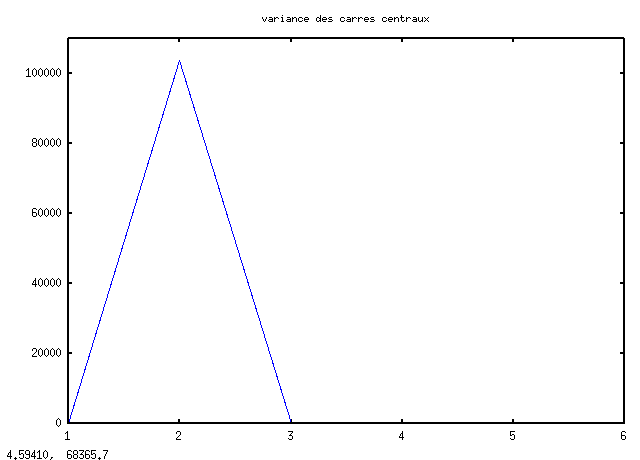
\includegraphics[width=0.5\linewidth]{./Images/var.png}
    \caption{Variance des carrés centraux}
    \label{fig:var}
   \end{figure}

  Nous pouvons constater que le centre de la face 2 a une variance beaucoup plus élevée que celle des autres. 
Ainsi nous modifions les valeurs RGB du centre mis en valeur à des valeurs correspondant à du blanc (255, 255, 255). 

  Ainsi sur des échantillons de photo prises sans reflet, on obtient avec des algorithmes tel que les K plus proches voisins (KPPV) ou le K-Means que nous avons implantés, le résultat de la figure~\ref{fig:RGBok}. 
  \begin{figure}[!ht]
    \centering
    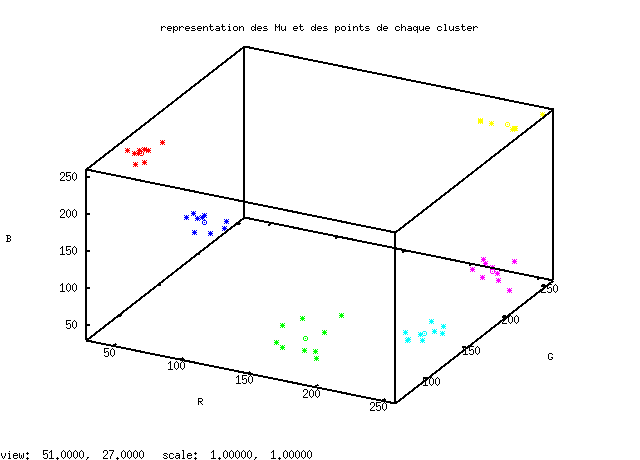
\includegraphics[width=0.5\linewidth]{./Images/RGB_ok.png}
    \caption{Variance des carrés centraux}
    \label{fig:RGBok}
   \end{figure}

  Nous obtenons bien 6 classes de 9 éléments. 


\subsection{Résolution par KNN}
  \subsubsection{Principe}

  Cette méthode est simple et nous a permis d'avoir un premier aperçu du rendu d'une classification. 

  Nous avons utilisé les données des centres pour créer notre modèle. 

  Ainsi les éléments vont être rattachés à la classe caractérisée par le centre le plus proche. 
Nous avons utilisé la distance euclidienne pour calculer la distance entre les éléments. 

  \subsubsection{Implantation initiale}

  Nous avons utilisé la toolbox créée en cours de Data Mining dont la signature est : 

  \verb|function [y_new] = kppv( x_new,x, y)|

  On utilise les valeurs de paramètres suivants : 
  \begin{itemize}
    \item x\_new = valeur RGB des carrés ;
    \item x = valeur RGB des centres ;
    \item y = label associé à chaque centre. 
  \end{itemize}

Les valeurs calculées sont : 
  \begin{itemize}
    \item y\_new = label des différents éléments de x. 
  \end{itemize}


\subsection{Résolution par KMeans}
\subsubsection{Principe}

  \begin{enumerate}
    \item On initialise autant de valeurs que de nombre de classes voulues, qui correspondent aux points de gravité des classes ;
    \item Les données sont placées dans les classes en fonction de leur proximité avec l'un ou l'autre des centres de gravité ; 
    \item Ces centres sont recalculés en fonction des données affectées à la classe ; 
    \item On refait les étapes 2 et 3 jusqu'à ce que les centres de gravité n'évolue plus. 
  \end{enumerate}

\subsubsection{Implantation initiale}

  Nous avons utilisé la toolbox crée en cours de Data Mining dont la signature est : 

  \verb|function [nouveauMu, z, er]=k_moyenne(X,nbCluster,nbIteration, epsilon, initMu )|

  On utilise les valeurs de paramètres suivants : 
  \begin{itemize}
    \item X = valeur RGB des carrés ;
    \item nbCluster  = 6 ; 
    \item nbIteration = 10 (valeur de conditions d'arrêt : nombre de centres de gravité successifs à calculer) ; 
    \item epsilon = 0.01 (valeur de conditions d'arrêt : variation entre les différentes valeurs successives des centres de gravité) ; 
    \item initMu = valeur RGB des centres. 
  \end{itemize}

Les valeurs calculées sont : 
  \begin{itemize}
    \item nouveauMu = dernières valeurs des centres de gravité calculées ; 
    \item z = label des différents éléments de X ; 
    \item er = erreur concernant le nombre d'élément par classe (0 si 9 éléments par classe, 1 sinon). 
  \end{itemize}

  Cette algorithme donne des résultats précis sur des photos ayant un bon éclairage mais nous devons ajouter une condition d'arrêt dans notre algorithme de résolution qui consiste à vérifier si on a bien 9 éléments dans chaque classe. 

\subsubsection{Utilisation de la conditions : ``9 carrés par classe''}

  Afin d'adapter l'algorithme à notre application, nous avons rajouté un traitement en cas d'erreur (er=1). 

  Ainsi on modifie les labels des éléments après le K-Mean de tel façon que les classes ayant plus de 9 éléments donnent successivement un de leurs éléments aux centres ayant un déficit d'éléments, le plus proche, jusqu'à ce que ces classes atteignent chacune 9 éléments. 

  Le résultat de classification obtenu est celui de la figure~\ref{RGBnok}
  \begin{figure}[h!]
    \centering
    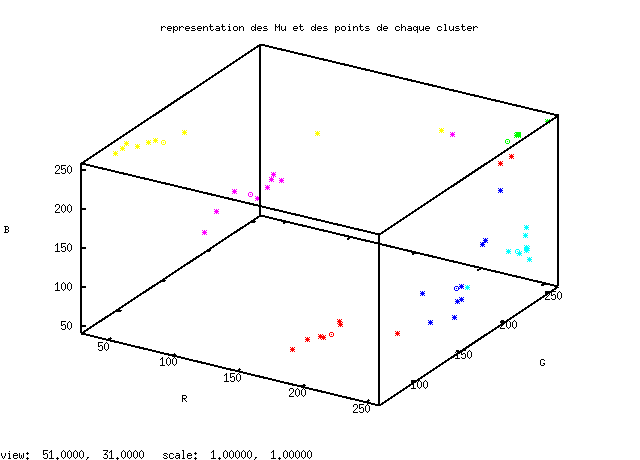
\includegraphics[width=0.5\linewidth]{./Images/RGB_nok.png}
    \caption{Représentation des données RGB des différents carrés}
    \label{RGBnok}
   \end{figure}

% \subsubsection{Limites}
% 
%   Comme il est visible sur la figure~\ref{RGBnok} sur la classe rouge notamment, les classes se retrouvent coupées en deux par d'autres classes. 
%   En effet, une classe qui a trop d'éléments peut donné un ou plusieurs de ceux-là à une classe qui est à l'opposé, si elle manque d'éléments. 
% 
% \subsubsection{Piste de résolution}
% 
%   Il faut mettre en place la condition concernant le nombre d'éléments par classe dans l'algorithme de résolution du K-Mean de tel façon que le rééquilibrage des classes se fassent entre les classes voisines. 


%%%%%%%%%%%%%%%%%%%%%%%%%%%%%%%%%%%%%%%%%%%%%%%%%%%%%%%%%%%%%%%%%%%%%%%%%%%%%%%%%
\section{Intégration au projet \rubic} % P4
  Nous avons mis en place un script bash qui permet de faire automatiquement une acquisition de photo et un traitement par notre algorithme de reconnaissance d'image. 

  Pour cela, il est nécessaire d'installer les logiciels cités ci-dessous et de brancher le boîtier NXJ et la caméra. 

  Le programme se lance grâce à l'exécutable COMPILEALL disponible à la racine de l'arborescence. 

  Ce programme effectue les étapes suivantes : 
  \begin{enumerate}
    \item Compilation des codes permettant de se connecter au boîtier NXJ, d'effectuer un mouvement avec le robot et de résoudre le cube. Dans notre cas, nous n'avons pas lancé directement la résolution du cube mais fait un affichage du résultat de l'initialisation comme montré dans la figure~\ref{fig:aff}.

    \item Capture des images du cube successive et déplacement du cube par le robot, 
    \item Utilisation de la reconnaissance d'image pour initialiser un cube. 
Le résultat de cette initialisation est sauvé dans un fichier, 
    \item Lecture de ce fichier par une classe Java intégrable dans la problématique générale du projet \rubic, 
    \item Affichage du résultat par la classe Java Main utilisé pour tester l'algorithme. 
  \end{enumerate}
    
  \begin{figure}[h!]
    \centering
    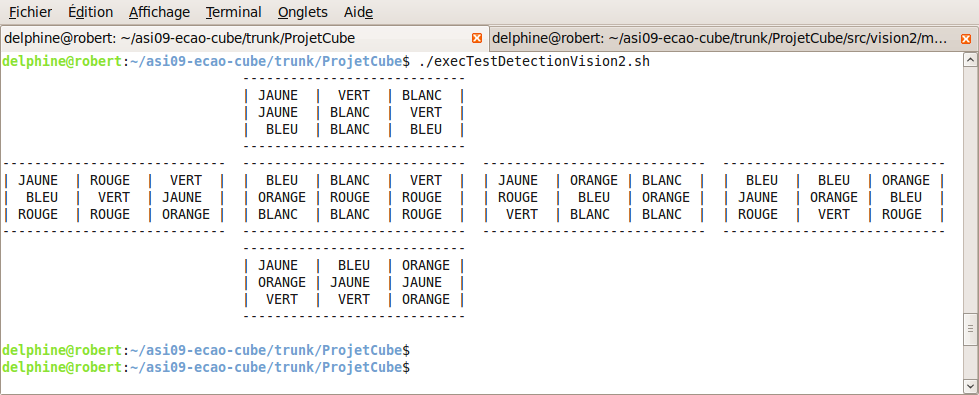
\includegraphics[width=0.8\linewidth]{./Images/affichage.png}
    \caption{Résultat de l'initialisation}
    \label{fig:aff}
   \end{figure}
  
  \textit{Remarque} Le résultat dans la figure~\ref{fig:aff} est obtenu à partir de la configuration 5 en Annexe~\ref{sec:Aconf}. 

  Le fichier permet la gestion des erreurs de détection de reflet et de détection de contour. 
  Ces erreurs sont traitées dans le programme Java qui récupère le résultat et provoque l'affichage de warning. 

  Nous n'avons pas ajouter la résolution du cube existante car nos résultats n'étaient pas satisfaisant, comme expliqué dans le chapitre~\ref{sec:avancement}. 

  \subsection*{Logiciels utilisés}

  Les logiciels à installer pour utiliser la reconnaissance d'image, en plus de ceux qui s'installent automatiquement grâce à instal.sh, sont : 
\begin{itemize}
  \item octave et octave-image pour l'algorithme de reconnaissance ; 
  \item gst pour la prise de photo ; 
  \item beep pour le signal sonore qui indique la fin de l'initialisation du cube est indique à l'utilisateur qu'il doit rallumer le boîtier NXJ pour la suite de la résolution du cube. En effet le temps de la reconnaissance d'image est suffisamment long pour que le boîtier NXJ s'éteigne, il faut alors le rallumer manuellement ; 
\end{itemize}

\textit{Remarque : } Si la caméra ne fonctionne pas, il est conseillé de baisser la résolution. 


%%%%%%%%%%%%%%%%%%%%%%%%%%%%%%%%%%%%%%%%%%%%%%%%%%%%%%%%%%%%%%%%%%%%%%%%%%%%%%%%%
\section{État actuel d'avancement de la partie vision} % P3 
\label{sec:avancement}
  A l'heure actuel, la partie vision du projet est fonctionnel, En effet nous avons mis en place une solution permettant de faire communiquer le code matlab précédemment produit avec le code java de l'ensemble du projet.
  Cependant, le taux de réussite de notre algorithme est très insatisfaisant. 

\subsection{Erreur de détection de contour}

\subsubsection{Problème principal}

	La principale raison de l'échec se situe au niveau de la détection des contours des faces colorés. Pour rappel, nous détectons quatre droites sur chacune des six faces du cube pour nous permettre d'obtenir les 54 facettes du cube.

	Or si le taux de réussite est acceptable pour la détection des facettes sur une seule face du cube, il devient très faible lors d'une détection sur les six faces.
	
\subsubsection{Causes principales}
	
	Notre algorithme se base sur la détection des arrêtes foncés du cube. Cependant l'ensemble des arrêtes sont brillantes, ce qui pose le problème suivant :
	Dans le cas d'un éclairage diffus, l'ensemble des arrêtes apparaissent noir, c'est le cas idéal. S'il existe une source de lumière directionnelle, certaines arrêtes apparaîtrons parfaitement blanches du fait de la brillance.
	
\subsubsection{Pistes de résolution}

	Dans le code actuel, nous somme capable de savoir si une erreur de détection s'est produite, auquel cas nous interrompons les calculs. Un solution relativement rapide à mettre en place serait de traiter ces erreur sur les axes suivants :
	\begin{itemize}
	\item Si au moins l'une des face est détectée correctement, alors il doit être possible d'appliquer la grille de détection sur l'ensemble des faces.
	\item Si sur une seule face, et pour une seule projection, les deux droites détectés ne sont pas celles attendus, alors il est possible d'en détecter une troisième dans le but d'obtenir les droites voulues.
	\end{itemize}	
	
\subsection{Erreur de détection de couleur}

\subsubsection{Problème principal}

  Comme il est visible sur la figure~\ref{RGBnok} sur la classe rouge notamment, les classes se retrouvent coupées en deux par d'autres classes. 
  En effet, avec la méthode implantée, une classe qui a trop d'éléments peut donné un ou plusieurs de ceux-là à une classe qui est à l'opposé, si elle manque d'éléments. 

%\subsubsection{Causes principales}

  
\subsubsection{Piste de résolution}

  Il faut mettre en place la condition concernant le nombre d'éléments par classe dans l'algorithme de résolution du K-Mean de tel façon que le rééquilibrage des classes se fassent entre les classes voisines. 

%%%%%%%%%%%%%%%%%%%%%%%%%%%%%%%%%%%%%%%%%%%%%%%%%%%%%%%%%%%%%%%%%%%%%%%%%%%%%%%%%
\section{Conclusion} % P5
\subsection{Présentation des résultats}

  Finalement, nous avons mis au point, d'une part, une reconnaissance d'image fonctionnelle sur la base de test que nous avions pour travailler, et qui gère les erreurs et, d'autre part, un système automatique permettant de prendre les photos des 6 faces, de les traiter pour initialiser un cube grâce à une fonction intégrable dans le programme Java original. 

  Les résultats obtenus sont ceux des figures~\ref{fig:res1} et ~\ref{fig:res2} qui sont la face 1 et la face 2 d'un cube. 
On observe que la figure~\ref{fig:res1} trouve bien les contours alors que dans la figure~\ref{fig:res2}, la ligne la plus basse de détection de contour (dessinée en noir) n'est pas celle que l'on espérai puisque l'on souhaite détecter les deux lignes séparatrices du milieu pour reconstruire la face du cube. 

  La cause de cette erreur est visible en comparant les courbes rouges qui correspondent aux projections en Y des images. 
On voit que les 2 pics minimaux ne sont pas les mêmes dans ces deux cas. 

  \begin{figure*}[!ht]
    \centering
    %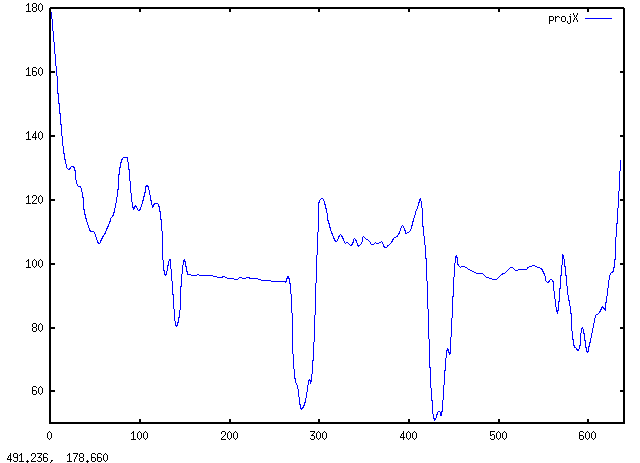
\includegraphics[width=0.4\linewidth]{./Images/projX_1.png}
    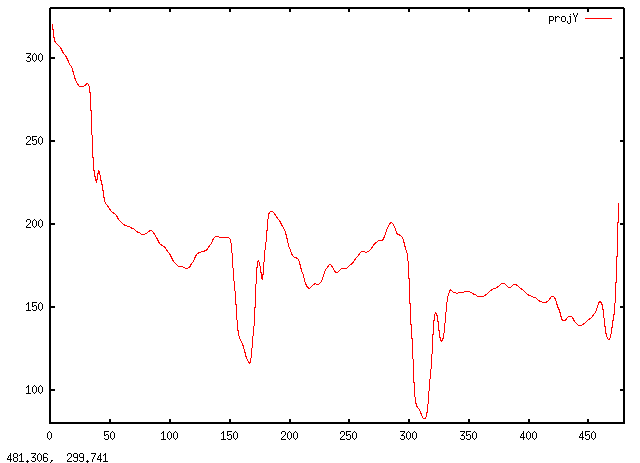
\includegraphics[width=0.4\linewidth]{./Images/projY_1.png}
    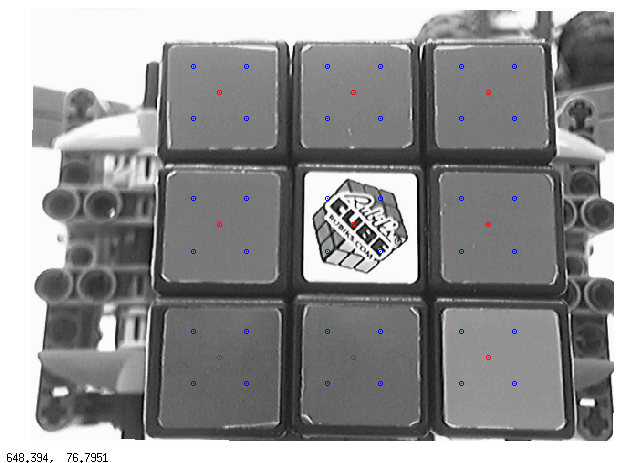
\includegraphics[width=0.4\linewidth]{./Images/face_1.png}
    \caption{Résultat sur une image sans reflet}
    \label{fig:res1}
   \end{figure*}

  \begin{figure*}[!ht]
    \centering
    %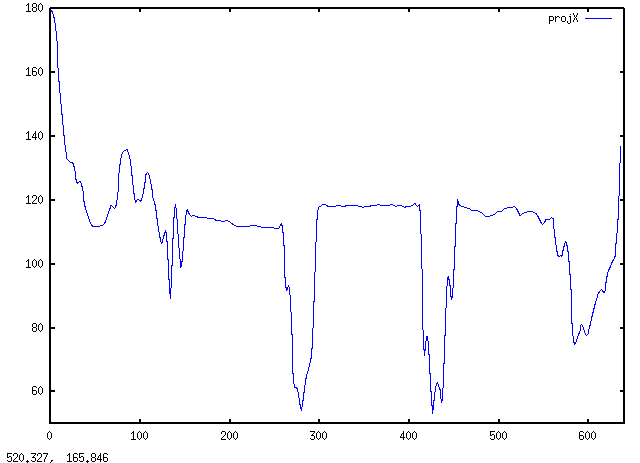
\includegraphics[width=0.4\linewidth]{./Images/projX_2.png}
    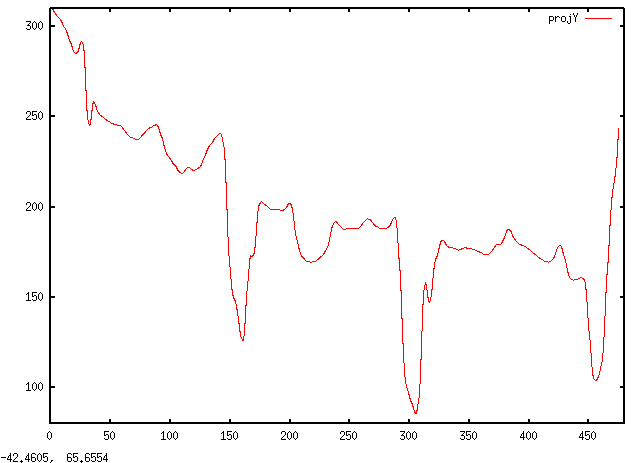
\includegraphics[width=0.4\linewidth]{./Images/projY_2.png}
    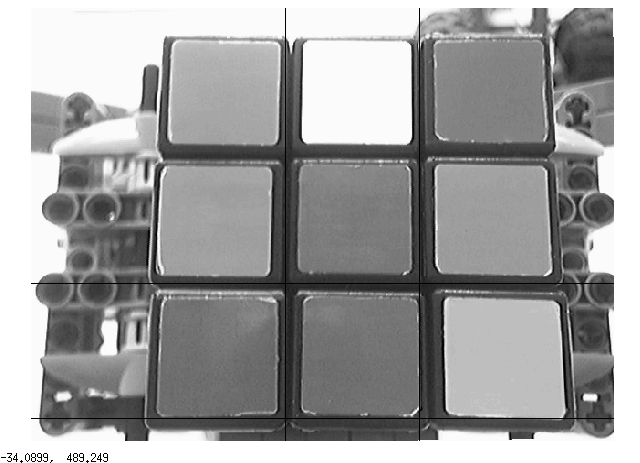
\includegraphics[width=0.4\linewidth]{./Images/face_2.png}
    \caption{Résultat sur une image avec reflet}
    \label{fig:res2}
   \end{figure*}

\textit{Remarque : } Les résultats des figures~\ref{fig:res1} et ~\ref{fig:res2} sont obtenus à partir de la configuration 0 en Annexe~\ref{sec:Aconf}. 

\subsection{Nos impressions}
Lorsque nous avons choisi cette ECAO, nous pensions que le problème posé était simple. Nous devions dans un premier temps mettre en place une série de tests sous matlab dans le but d'intégrer la meilleur solution en java. Cependant au cours de nos expériences, nous nous sommes heurtés à plusieurs problèmes successifs tel que la prise en compte de la couleur de certaines pièces du robot, ou les conditions d'éclairage. 

Notre approche de segmentation a eu pour but de segmenter l'image de la façon suivante : nous détectons 2 lignes noir horizontales et 2 lignes noir verticale pour en déduire la positions de chacune des 9 facettes. Cette approche avait pour but de transformer le problème en un cas particulièrement simple. Ainsi nous pouvions écarter facilement le bruit et éviter l'utilisation d'algorithmes beaucoup plus lourds comme de la reconnaissance de formes. 

Suites à nos résultats, nous remettons partiellement en cause cette approche. En effet, nous n'avons de ce fait pas étudié les résultats d'algorithmes de segmentations classiques qui nous auraient peut-être donnés de meilleurs résultats.

  Cependant, cette ECAO nous a permis de comprendre la complexité des problématiques liées à l'étude d'image. Elle nous a permis de faire appel à plusieurs compétences : vision, data mining, programmation matlab et Java, c'est un projet riche ainsi qu'il faudrait segmenter pour le mener à bien. 


%%%%%%%%%%%%%%%%%%%%%%%%%%%%%%%%%%%%%%%%%%%%%%%%%%%%%%%%%%%%%%%%%%%%%%%%%%%%%%%%%
\section{Annexes}

\subsection{Fonctions Octave}
Afin de rendre notre code compréhensible, nous avons fait un inventaire des fonctions proposées 
par Octave que nous avons eu à utiliser : 

\begin{center} 
\begin{tabular}{|c|c|}
  \hline 
    diff & calcul la dérivée du vecteur en entrée \\
    &(la dérivée a une valeur de moins que le vecteur en entrée)\\
  \hline 
    sign & retourne un vecteur contenant\\
    & 1 si la valeur en entrée est positive\\
    & -1 si la valeur en entrée est negative\\
  \hline 
    find & retourne les indices tel que la condition en entrée soit vrai\\
    &(cette condition concerne souvent des vecteurs)\\
  \hline 
    min, max & \\
  \hline 
    abs & \\
  \hline 
\end{tabular}
\end{center}


\subsection{Jeux d'images utilisés}
\label{sec:Aconf}
  \begin{figure*}[!ht]
    \centering
    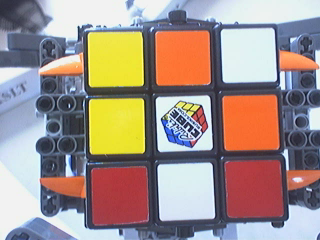
\includegraphics[width=0.4\linewidth]{../image/conf5/face1.png}
    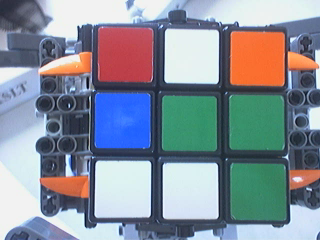
\includegraphics[width=0.4\linewidth]{../image/conf5/face2.png}
    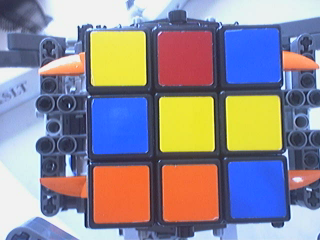
\includegraphics[width=0.4\linewidth]{../image/conf5/face3.png}
    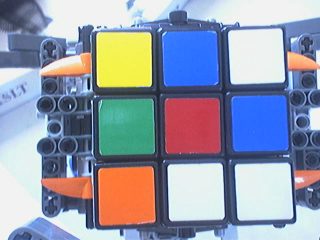
\includegraphics[width=0.4\linewidth]{../image/conf5/face4.png}
    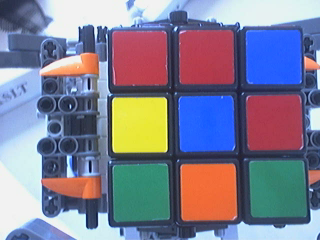
\includegraphics[width=0.4\linewidth]{../image/conf5/face5.png}
    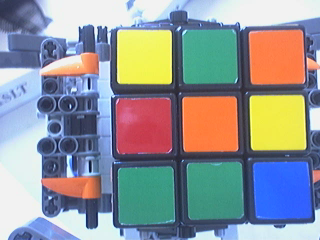
\includegraphics[width=0.4\linewidth]{../image/conf5/face6.png}
    \caption{Configuration numéro 5 : bonne condition d'éclairage}
    \label{fig:conf5}
   \end{figure*}

  \begin{figure*}[!ht]
    \centering
    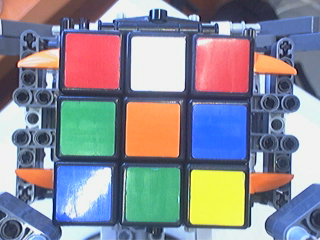
\includegraphics[width=0.4\linewidth]{../image/conf7/face1.png}
    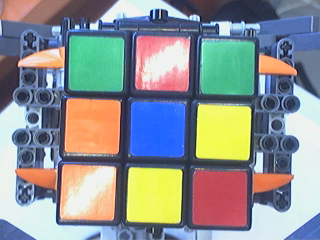
\includegraphics[width=0.4\linewidth]{../image/conf7/face2.png}
    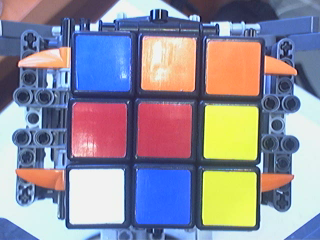
\includegraphics[width=0.4\linewidth]{../image/conf7/face3.png}
    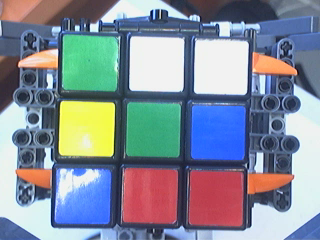
\includegraphics[width=0.4\linewidth]{../image/conf7/face4.png}
    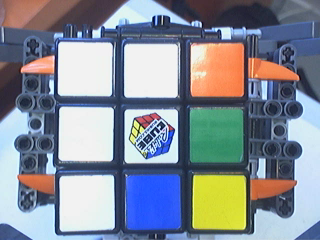
\includegraphics[width=0.4\linewidth]{../image/conf7/face5.png}
    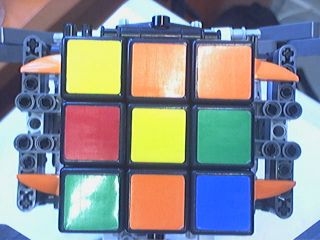
\includegraphics[width=0.4\linewidth]{../image/conf7/face6.png}
    \caption{Configuration numéro 7 : erreur de reflets}
    \label{fig:conf7}
   \end{figure*}

  \begin{figure*}[!ht]
    \centering
    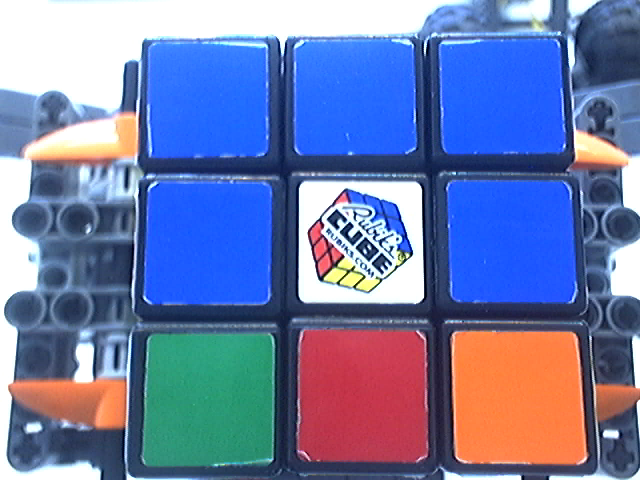
\includegraphics[width=0.4\linewidth]{../image/conf0/face1.png}
    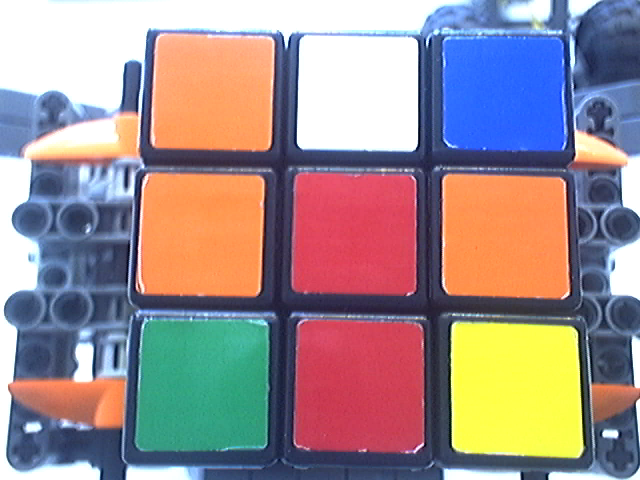
\includegraphics[width=0.4\linewidth]{../image/conf0/face2.png}
    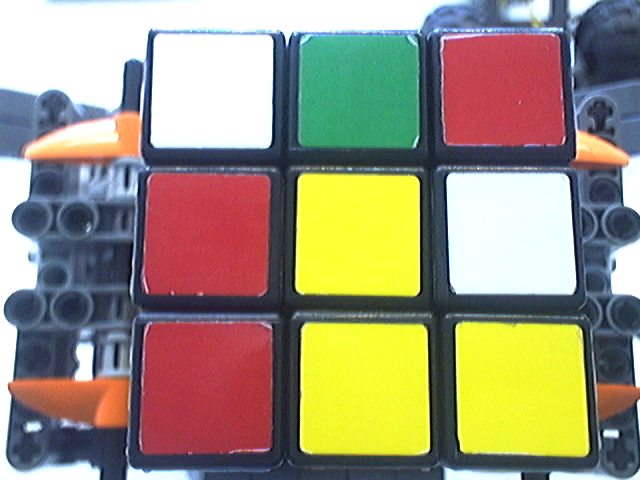
\includegraphics[width=0.4\linewidth]{../image/conf0/face3.png}
    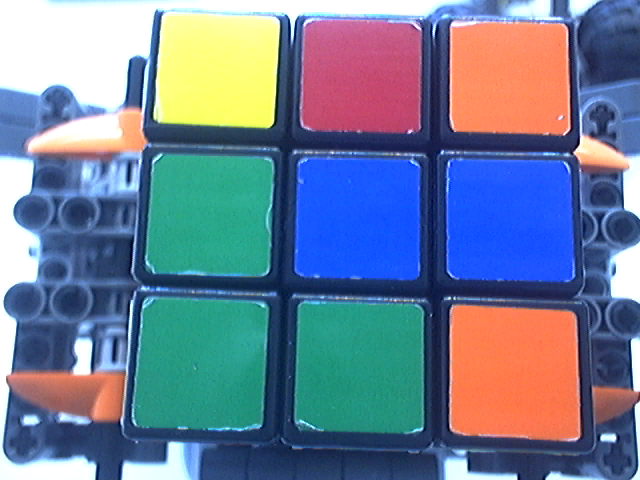
\includegraphics[width=0.4\linewidth]{../image/conf0/face4.png}
    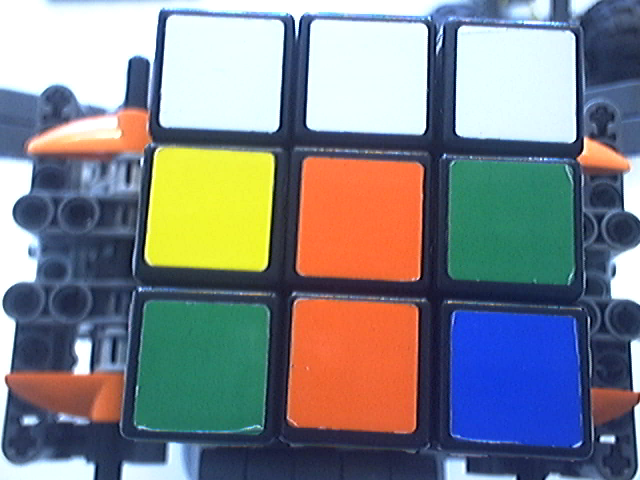
\includegraphics[width=0.4\linewidth]{../image/conf0/face5.png}
    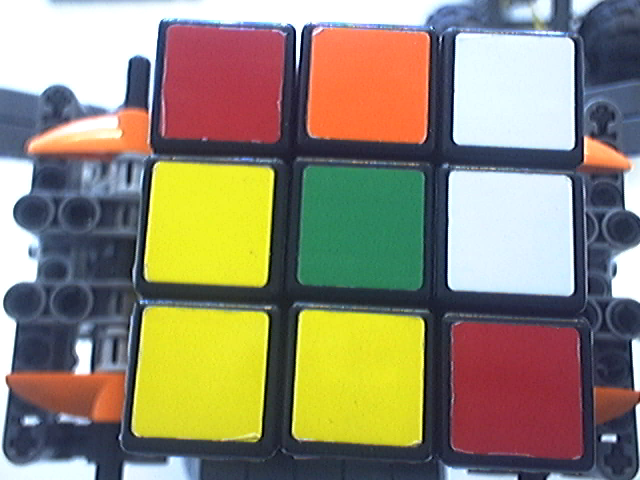
\includegraphics[width=0.4\linewidth]{../image/conf0/face6.png}
    \caption{Configuration numéro 0 : erreur de contours}
    \label{fig:conf0}
   \end{figure*}


\end{document}
